\documentclass[tikz,border=4pt]{standalone}

\usepackage[T1]{fontenc}
\renewcommand{\rmdefault}{ptm}
\usetikzlibrary{arrows.meta,positioning}

\definecolor{Ink}{HTML}{1F2937}
\definecolor{DataFill}{HTML}{EDF1F4}
\definecolor{DataEdge}{HTML}{4F5D6B}
\definecolor{ProcessFill}{HTML}{E8F1F7}
\definecolor{ProcessEdge}{HTML}{2A6F9E}
\definecolor{ModelFill}{HTML}{F8EBDD}
\definecolor{ModelEdge}{HTML}{B85C1E}
\definecolor{OpticsFill}{HTML}{EAF2EC}
\definecolor{OpticsEdge}{HTML}{4F7A5A}

\tikzset{
  data panel/.style={draw=DataEdge, fill=DataFill, rounded corners=3.0pt, line width=0.9pt},
  process panel/.style={draw=ProcessEdge, fill=ProcessFill, rounded corners=3.0pt, line width=0.9pt},
  model panel/.style={draw=ModelEdge, fill=ModelFill, rounded corners=3.0pt, line width=0.9pt},
  optics panel/.style={draw=OpticsEdge, fill=OpticsFill, rounded corners=3.0pt, line width=0.9pt},
  stage title/.style={font=\rmfamily\bfseries\fontsize{8.2}{9.2}\selectfont, align=center},
  stage step/.style={font=\rmfamily\fontsize{7.2}{8.2}\selectfont, align=center, text=Ink,
    text width=2.55cm, inner sep=0pt},
  outer flow/.style={-{Latex[length=1.9mm,width=1.3mm]}, draw=Ink, line width=0.85pt},
  inner flow/.style={-{Latex[length=1.35mm,width=0.95mm]}, draw=Ink, line width=0.65pt},
}

\begin{document}
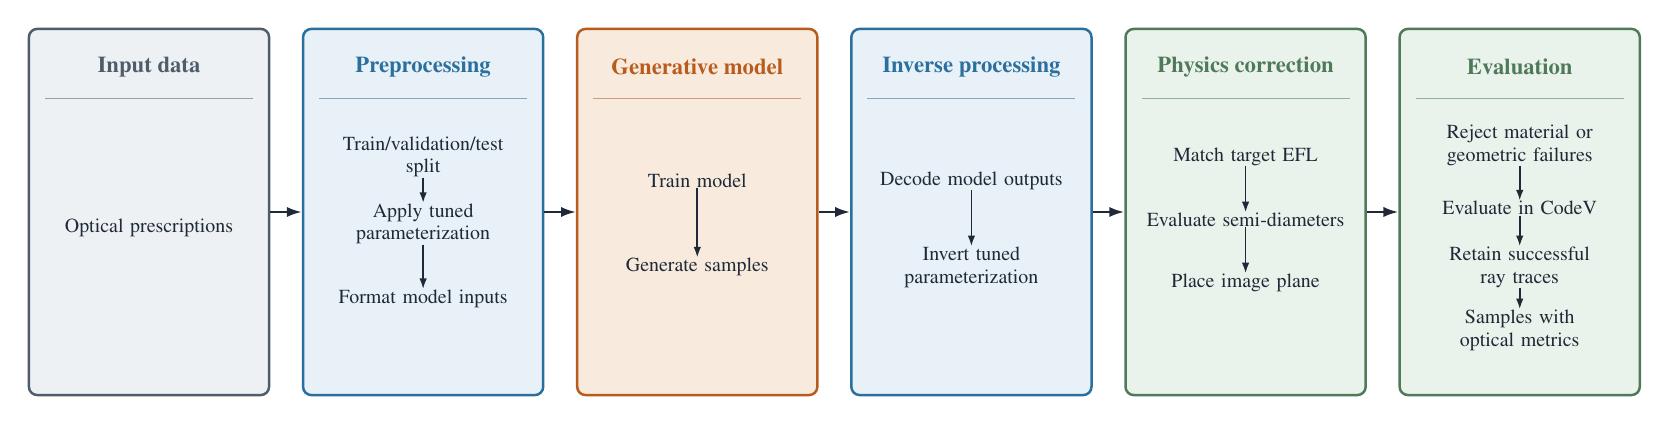
\begin{tikzpicture}[node distance=4.0mm]
  % Equal-size stage panels preserve a regular horizontal rhythm.
  \node[data panel, minimum width=3.05cm, minimum height=4.65cm] (data) {};
  \node[process panel, minimum width=3.05cm, minimum height=4.65cm, right=of data] (pre) {};
  \node[model panel, minimum width=3.05cm, minimum height=4.65cm, right=of pre] (model) {};
  \node[process panel, minimum width=3.05cm, minimum height=4.65cm, right=of model] (inverse) {};
  \node[optics panel, minimum width=3.05cm, minimum height=4.65cm, right=of inverse] (physics) {};
  \node[optics panel, minimum width=3.05cm, minimum height=4.65cm, right=of physics] (evaluation) {};

  % Stage titles and restrained title dividers.
  \node[stage title, text=DataEdge] at ([yshift=-5.0mm]data.north) {Input data};
  \node[stage title, text=ProcessEdge] at ([yshift=-5.0mm]pre.north) {Preprocessing};
  \node[stage title, text=ModelEdge] at ([yshift=-5.0mm]model.north) {Generative model};
  \node[stage title, text=ProcessEdge] at ([yshift=-5.0mm]inverse.north) {Inverse processing};
  \node[stage title, text=OpticsEdge] at ([yshift=-5.0mm]physics.north) {Physics correction};
  \node[stage title, text=OpticsEdge] at ([yshift=-5.0mm]evaluation.north) {Evaluation};

  \draw[DataEdge, line width=0.45pt, opacity=0.55]
    ([xshift=2.2mm,yshift=-9.0mm]data.north west) -- ([xshift=-2.2mm,yshift=-9.0mm]data.north east);
  \draw[ProcessEdge, line width=0.45pt, opacity=0.55]
    ([xshift=2.2mm,yshift=-9.0mm]pre.north west) -- ([xshift=-2.2mm,yshift=-9.0mm]pre.north east);
  \draw[ModelEdge, line width=0.45pt, opacity=0.55]
    ([xshift=2.2mm,yshift=-9.0mm]model.north west) -- ([xshift=-2.2mm,yshift=-9.0mm]model.north east);
  \draw[ProcessEdge, line width=0.45pt, opacity=0.55]
    ([xshift=2.2mm,yshift=-9.0mm]inverse.north west) -- ([xshift=-2.2mm,yshift=-9.0mm]inverse.north east);
  \draw[OpticsEdge, line width=0.45pt, opacity=0.55]
    ([xshift=2.2mm,yshift=-9.0mm]physics.north west) -- ([xshift=-2.2mm,yshift=-9.0mm]physics.north east);
  \draw[OpticsEdge, line width=0.45pt, opacity=0.55]
    ([xshift=2.2mm,yshift=-9.0mm]evaluation.north west) -- ([xshift=-2.2mm,yshift=-9.0mm]evaluation.north east);

  % Stage contents are unboxed to keep the hierarchy visually quiet.
  \node[stage step] at ([yshift=-2.0mm]data.center) {Optical prescriptions};

  \node[stage step] (split) at ([yshift=7.0mm]pre.center) {Train/validation/test split};
  \node[stage step] (parameterize) at ([yshift=-1.5mm]pre.center) {Apply tuned\\parameterization};
  \node[stage step] (format) at ([yshift=-11.0mm]pre.center) {Format model inputs};

  \node[stage step] (train) at ([yshift=4.0mm]model.center) {Train model};
  \node[stage step] (sample) at ([yshift=-7.0mm]model.center) {Generate samples};

  \node[stage step] (decode) at ([yshift=4.0mm]inverse.center) {Decode model outputs};
  \node[stage step] (invert) at ([yshift=-7.0mm]inverse.center) {Invert tuned\\parameterization};

  \node[stage step] (efl) at ([yshift=7.0mm]physics.center) {Match target EFL};
  \node[stage step] (diameters) at ([yshift=-1.0mm]physics.center) {Evaluate semi-diameters};
  \node[stage step] (image) at ([yshift=-9.0mm]physics.center) {Place image plane};

  \node[stage step] (reject) at ([yshift=8.5mm]evaluation.center) {Reject material or\\geometric failures};
  \node[stage step] (codev) at ([yshift=0.5mm]evaluation.center) {Evaluate in CodeV};
  \node[stage step] (success) at ([yshift=-7.0mm]evaluation.center) {Retain successful\\ray traces};
  \node[stage step] (metrics) at ([yshift=-15.0mm]evaluation.center) {Samples with\\optical metrics};

  % Internal and inter-stage flow remains explicit and directional.
  \draw[inner flow] (split.south) -- (parameterize.north);
  \draw[inner flow] (parameterize.south) -- (format.north);
  \draw[inner flow] (train.south) -- (sample.north);
  \draw[inner flow] (decode.south) -- (invert.north);
  \draw[inner flow] (efl.south) -- (diameters.north);
  \draw[inner flow] (diameters.south) -- (image.north);
  \draw[inner flow] (reject.south) -- (codev.north);
  \draw[inner flow] (codev.south) -- (success.north);
  \draw[inner flow] (success.south) -- (metrics.north);

  \draw[outer flow] (data.east) -- (pre.west);
  \draw[outer flow] (pre.east) -- (model.west);
  \draw[outer flow] (model.east) -- (inverse.west);
  \draw[outer flow] (inverse.east) -- (physics.west);
  \draw[outer flow] (physics.east) -- (evaluation.west);
\end{tikzpicture}
\end{document}
